\documentclass{amsart}
\usepackage{amssymb,enumerate,bbm,amsmath}
\usepackage[colorlinks=true,linkcolor=blue,citecolor=blue]{hyper ref}
\usepackage{tikz}

\begin{document}

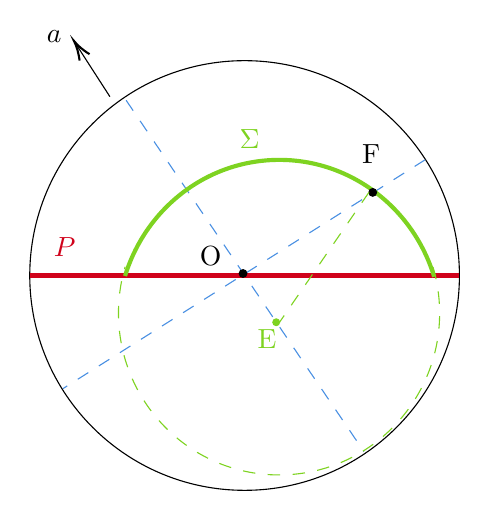
\begin{tikzpicture}[x=0.70pt,y=0.70pt,yscale=-0.93,xscale=0.93]
				
				\draw   (203,154.25) .. controls (203,88.39) and (256.39,35) .. (322.25,35) .. controls (388.11,35) and (441.5,88.39) .. (441.5,154.25) .. controls (441.5,220.11) and (388.11,273.5) .. (322.25,273.5) .. controls (256.39,273.5) and (203,220.11) .. (203,154.25) -- cycle ;
				\draw [color={rgb, 255:red, 208; green, 2; blue, 27 }  ,draw opacity=1 ][line width=1.5]    (203,154.25) -- (441.5,154.25) ;
				\draw [color={rgb, 255:red, 74; green, 144; blue, 226 }  ,draw opacity=1 ] [dash pattern={on 4.5pt off 4.5pt}]  (422.5,90) -- (221.5,217) ;
				\draw [color={rgb, 255:red, 74; green, 144; blue, 226 }  ,draw opacity=1 ] [dash pattern={on 4.5pt off 4.5pt}]  (256.5,57) -- (388.5,252) ;
				\draw  [draw opacity=0][line width=1.5]  (255.9,154.53) .. controls (266.95,118.27) and (299.4,91.44) .. (338.58,90.12) .. controls (379.97,88.74) and (415.79,116.27) .. (427.47,154.96) -- (341.66,182.07) -- cycle ; \draw  [color={rgb, 255:red, 126; green, 211; blue, 33 }  ,draw opacity=1 ][line width=1.5]  (255.9,154.53) .. controls (266.95,118.27) and (299.4,91.44) .. (338.58,90.12) .. controls (379.97,88.74) and (415.79,116.27) .. (427.47,154.96) ;  
				\draw  [draw opacity=0][dash pattern={on 4.5pt off 4.5pt}] (426.83,149.56) .. controls (429.09,157.25) and (430.37,165.38) .. (430.5,173.79) .. controls (431.26,223.38) and (391.98,264.19) .. (342.76,264.95) .. controls (293.54,265.7) and (253.02,226.12) .. (252.26,176.53) .. controls (252.11,167.1) and (253.41,157.99) .. (255.96,149.41) -- (341.38,175.16) -- cycle ; \draw  [color={rgb, 255:red, 126; green, 211; blue, 33 }  ,draw opacity=1 ][dash pattern={on 4.5pt off 4.5pt}] (426.83,149.56) .. controls (429.09,157.25) and (430.37,165.38) .. (430.5,173.79) .. controls (431.26,223.38) and (391.98,264.19) .. (342.76,264.95) .. controls (293.54,265.7) and (253.02,226.12) .. (252.26,176.53) .. controls (252.11,167.1) and (253.41,157.99) .. (255.96,149.41) ;  
				\draw    (247.5,55) -- (228.58,25.68) ;
				\draw [shift={(227.5,24)}, rotate = 57.17] [color={rgb, 255:red, 0; green, 0; blue, 0 }  ][line width=0.75]    (10.93,-3.29) .. controls (6.95,-1.4) and (3.31,-0.3) .. (0,0) .. controls (3.31,0.3) and (6.95,1.4) .. (10.93,3.29)   ;
				\draw  [color={rgb, 255:red, 126; green, 211; blue, 33 }  ,draw opacity=1 ][fill={rgb, 255:red, 126; green, 211; blue, 33 }  ,fill opacity=1 ] (337.91,180.19) .. controls (337.91,179.16) and (338.75,178.32) .. (339.79,178.32) .. controls (340.82,178.32) and (341.66,179.16) .. (341.66,180.19) .. controls (341.66,181.23) and (340.82,182.07) .. (339.79,182.07) .. controls (338.75,182.07) and (337.91,181.23) .. (337.91,180.19) -- cycle ;
				\draw  [fill={rgb, 255:red, 0; green, 0; blue, 0 }  ,fill opacity=1 ] (319.25,153.13) .. controls (319.25,151.95) and (320.2,151) .. (321.38,151) .. controls (322.55,151) and (323.5,151.95) .. (323.5,153.13) .. controls (323.5,154.3) and (322.55,155.25) .. (321.38,155.25) .. controls (320.2,155.25) and (319.25,154.3) .. (319.25,153.13) -- cycle ;
				\draw  [fill={rgb, 255:red, 0; green, 0; blue, 0 }  ,fill opacity=1 ] (391.25,108.13) .. controls (391.25,106.95) and (392.2,106) .. (393.38,106) .. controls (394.55,106) and (395.5,106.95) .. (395.5,108.13) .. controls (395.5,109.3) and (394.55,110.25) .. (393.38,110.25) .. controls (392.2,110.25) and (391.25,109.3) .. (391.25,108.13) -- cycle ;
				\draw [color={rgb, 255:red, 126; green, 211; blue, 33 }  ,draw opacity=1 ] [dash pattern={on 4.5pt off 4.5pt}]  (391.25,108.13) -- (341.66,180.19) ;
				
				% Text Node
				\draw (211,17) node [anchor=north west][inner sep=0.75pt]   [align=left] {$\displaystyle a$};
				% Text Node
				\draw (328,183) node [anchor=north west][inner sep=0.75pt]  [color={rgb, 255:red, 126; green, 211; blue, 33 }  ,opacity=1 ] [align=left] {E};
				% Text Node
				\draw (296,137) node [anchor=north west][inner sep=0.75pt]   [align=left] {O};
				% Text Node
				\draw (386,80) node [anchor=north west][inner sep=0.75pt]   [align=left] {F};
				% Text Node
				\draw (215,132) node [anchor=north west][inner sep=0.75pt]  [color={rgb, 255:red, 208; green, 2; blue, 27 }  ,opacity=1 ] [align=left] {$\displaystyle P$};
				% Text Node
				\draw (318,72) node [anchor=north west][inner sep=0.75pt]  [color={rgb, 255:red, 126; green, 211; blue, 33 }  ,opacity=1 ] [align=left] {$\displaystyle \Sigma $};
				
				
			\end{tikzpicture}

\end{document}